\chapter{考察}\label{cha:Discussion}
本研究では、HTMLコードの差分とレイアウトの差分における整合性の確認にかかる時間の削減を目的として、
レイアウトの不具合箇所の可視化機能を持つ視覚的回帰テストツール\toolName を試作した。
本章では、
評価実験を行い、\toolName の有用性を評価する。
次に、\toolName と関連研究を比較する。
最後に、\toolName の問題点とその解決策について述べる。

\section{評価実験}
評価実験では、HTMLコードの差分とレイアウトの差分における整合性の確認にかかる時間に対する評価を行う。
具体的には、\toolName を使用した場合と、一般的な画像ベースの視覚的回帰テストで生成する差分画像を使用する場合とで、
目視によるレイアウトの不具合箇所の発見にかかる時間を、それぞれ計測する。
なお、\toolName を使用する場合をCaseA、一般的な画像ベースの視覚的回帰テストで生成する差分画像を使用する場合をCaseB
とする。

CaseAでは、
\toolName の実行完了後から、被験者がレイアウトの不具合箇所を見つけるまでにかかった時間を発見時間として計測する。
CaseBでは、
変更前後のWebページの差分画像を見てから、被験者がレイアウトの不具合箇所を見つけるまでにかかった時間を発見時間として計測する。


実験の事前準備として、HTMLコードで記述された実験用Webページを2つ作成し、それぞれ変更前と変更後のHTMLコードを用意する。
なお、2つの実験用Webページについて、変更後のWebページには、それぞれ3個のレイアウトの不具合箇所を埋め込む。
1つ目のWebページは、架空の大学サイトのWebページである。これを、サイトAと定義する。
2つ目のWebページは、架空のツール紹介サイトのWebページである。これを、サイトBと定義する。
実験に使用するWebページの例として、変更前後のサイトAを、
図\ref{fig:test1}に示す。
\begin{figure}[tp]
    \centering
    % 画像ファイル名とサイズを指定
    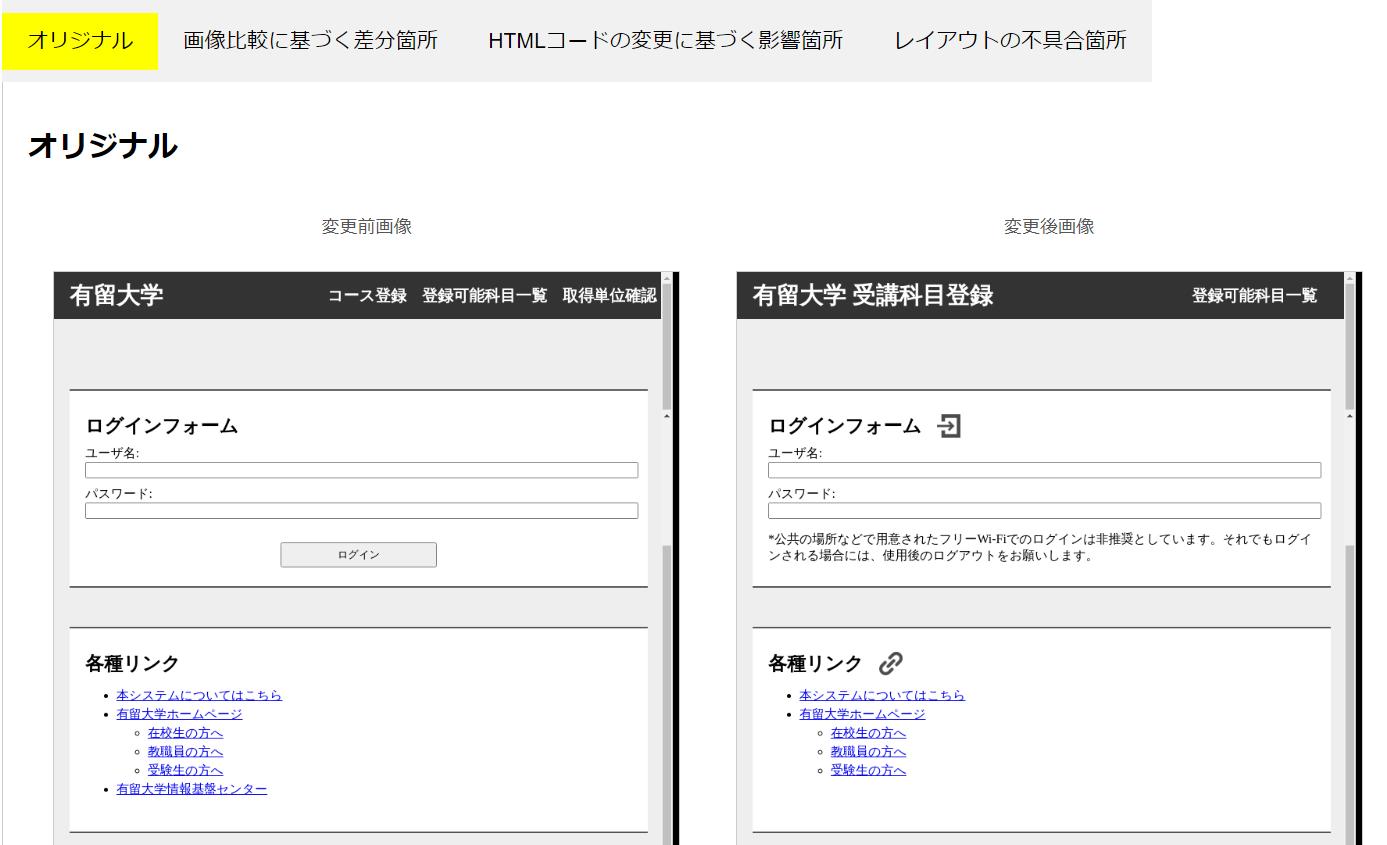
\includegraphics[width=1.0\textwidth]{image/original_test.png}
    \caption{実験に使用する変更前後のサイトA}
    \label{fig:test1}
\end{figure}
実験に参加する被験者は、宮崎大学で情報工学を専攻する4人の学生(以降、A~Dと呼ぶ)である。
実験を行う際には、実験用Webページの変更前画像と変更後画像を見ることができ、
また、実験用Webページの変更前HTMLコードと変更後HTMLコードも見ることができる。
さらに、被験者がレイアウトの不具合箇所を見つけた際に、その不具合箇所の位置を記録しておくための実験用ファイルも用意する。
% 被験者の中には、Webに関する知識がない者も含まれるが、今回は事前に説明する。
% 実験では、【実験によって\toolName が達成したいことを満たせているかを確認するためにこのような作業を提示する】。
% 以降、各作業の内容と結果を説明する。
\par
CaseAでは被験者は、図\ref{fig:test1_subeffect}に示した
\toolName のレイアウトの不具合箇所表示を用いて、
レイアウトの不具合箇所を確認する。
被験者が全てのレイアウトの不具合箇所を実験用ファイルに書き込み終えた場合に、実験を終了する。
\begin{figure}[tp]
    \centering
    % 画像ファイル名とサイズを指定
    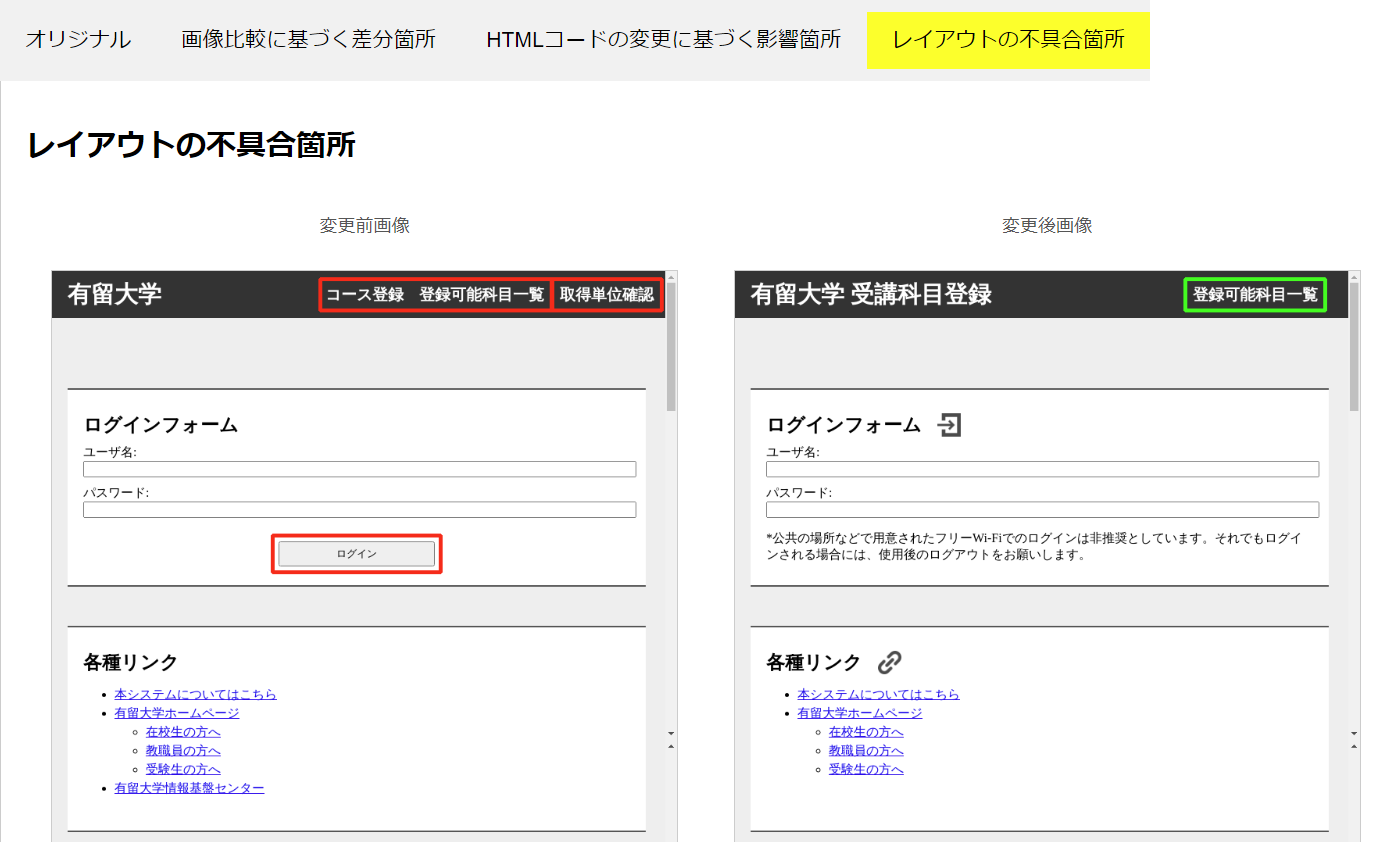
\includegraphics[width=1.0\textwidth]{image/5/5_app_3.png}
    \caption{レイアウトの不具合箇所表示}
    \label{fig:test1_subeffect}
\end{figure}

CaseBでは被験者は、図\ref{fig:test1_img}に示した\toolName の画像比較に基づく差分箇所表示を用いて、
レイアウトの不具合箇所を見つける。また、実験用Webページの変更前HTMLコードと変更後HTMLコードも確認することで、
画像比較に基づく差分箇所が、レイアウトの不具合箇所であるかどうかを判定する。
見つけたレイアウトの不具合箇所は実験用ファイルに書き込んでもらい、被験者が全てのレイアウトの不具合箇所を見つけたと判断したら実験を終了する。
\begin{figure}[tp]
    \centering
    % 画像ファイル名とサイズを指定
    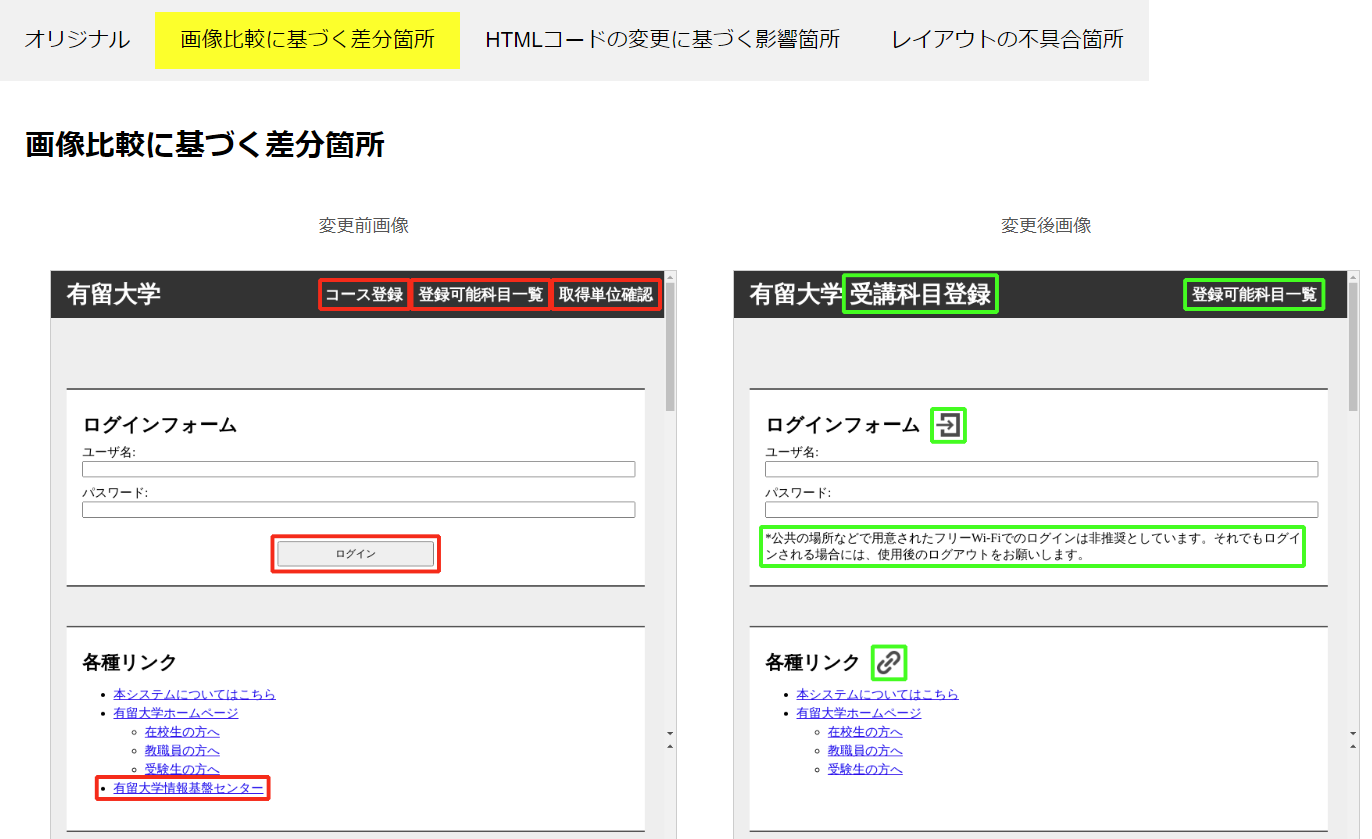
\includegraphics[width=1.0\textwidth]{image/5/5_app2.png}
    \caption{画像比較に基づく差分箇所表示}
    \label{fig:test1_img}
\end{figure}
CaseBにおけるレイアウトの不具合箇所を見つける流れについて、以下に示す。
\begin{enumerate}
    \item 画像比較に基づく差分箇所表示で、変更前画像上の全ての赤枠に対して、以下の操作を繰り返す。
          \begin{enumerate}
              \item 赤枠内の画面要素が、実験用Webページの変更後HTMLコードに存在しない、または、CSSクラスの変更を受けている場合、その画面要素は削除、または、変更されたと判定し、次の赤枠の確認に進む。
              \item 上記のそれ以外の場合、その画面要素は削除されていないと判定する。この場合、レイアウトの不具合箇所であるため、実験用ファイルに記録を取る。
          \end{enumerate}
    \item 画像比較に基づく差分箇所表示で、変更後画像上の全ての緑枠に対して、以下の判定を繰り返す。
          \begin{enumerate}
              \item 緑枠内の画面要素が、実験用Webページの変更前HTMLコードに存在しない、または、CSSクラスの変更を受けている場合、その画面要素は追加されたと判定し、次の緑枠の確認に進む。
              \item 上記のそれ以外の場合、その画面要素は追加されていないと判定する。この場合、レイアウトの不具合箇所であるため、実験用ファイルに記録を取る。
          \end{enumerate}
\end{enumerate}


\section{レイアウトの不具合箇所の発見時間に関する評価}\label{subsec:evalue_required_time}
レイアウトの不具合箇所を発見するのにかかった時間についての実験結果を、表\ref{fig: 6_1}に示す。
% 被験者Aは、大学ページを手動で16m 16s、Ariをツールで39s。
% 被験者Bは、大学ページをツールで1m 3s、Ariを手動で13m 40s。
% 被験者Cは、大学ページを手動で11m 54s、Ariをツールで48s。
% 被験者Dは、大学ページをツールで2m 37s、Ariを手動で12m 45s。

表\ref{fig: 6_1}から、\toolName を使用することで、発見時間を平均で12分22秒(90.6\%)削減することができた。
\toolName を使用することで、発見時間を削減できた要因として、CaseBでは差分画像のみしか被験者に提示できないところを、
CaseAではレイアウトの不具合箇所を可視化した画像を
被験者に提示したためであると考える。これにより、\toolName を用いた視覚的回帰テストでは、
レイアウトの変更があった箇所に対して、
HTMLコードを確認してレイアウトの不具合箇所かどうかを確認する手間を削減できたといえる。
よって、\toolName は、レイアウトの不具合箇所の発見にかかる時間の削減に有用である。

\begin{table}[h]
    \centering
    \caption{レイアウトの不具合箇所の発見時間についての実験結果}
    \label{fig: 6_1}
    \begin{tabular}{c||c|c|c|c}
               & \multicolumn{2}{|c|}{\textbf{サイトA}}
               & \multicolumn{2}{|c}{\textbf{サイトB}}                              \\
        \hline \hline
        被験者 & CaseA                                  & CaseB  & CaseA & CaseB    \\
        \hline \hline
        A      & -                                      & 16m16s & 39s   & -        \\
        B      & -                                      & 11m54s & 48s   & -        \\
        C      & 1m3s                                   & -      & -     & 13m40s   \\
        D      & 2m37s                                  & -      & -     & 12m45s   \\
        \hline
        平均   & 1m50s                                  & 14m5s  & 43.5s & 13m12.5s \\
    \end{tabular}
\end{table}


\section{レイアウトの不具合箇所の検出精度に関する評価}\label{subsec:evalue_accuracy}
評価実験において、CaseBで、被験者が
レイアウトの不具合箇所を過剰に検出することや、検出が不足することがあった。
それに対して、CaseAでは、
レイアウトの不具合箇所を過剰に検出することなく、また、不足なく検出することができた。
つまり、CaseAはレイアウトの不具合箇所を過不足なく検出できた。

CaseBにおけるレイアウトの不具合箇所を過剰に検出した数と、検出が不足した数を、表\ref{tb:result_detect}に示す。
なお、表\ref{tb:result_detect}における不具合箇所は、サイトに埋め込んだレイアウトの不具合箇所の総数を意味する。
\begin{table}[ht]
    \centering
    \caption{CaseBにおけるレイアウトの不具合箇所を過剰に検出した数と検出が不足した数}
    \label{tb:result_detect}
    \begin{tabular}{c||c|c|c|c|c}
        サイト                   & 不具合箇所         & 被験者 & 過剰 & 不足 & \\
        \hline \hline
        \multirow{2}{*}{サイトA} & \multirow{2}{*}{3} & A      & 0    & 0    & \\
        \cline{3-6}
                                 &                    & B      & 0    & 2    & \\
        \hline
        \multirow{2}{*}{サイトB} & \multirow{2}{*}{3} & C      & 1    & 1    & \\
        \cline{3-6}
                                 &                    & D      & 2    & 1    & \\
        \hline \hline
    \end{tabular}
\end{table}

CaseBで被験者がレイアウトの不具合箇所を過剰に検出したことについて、考察する。
被験者CとDは、
見た目の変更があった画面要素に対して、HTMLコードに基づく変更がされていたかどうかの
判定を誤ったため、レイアウトの不具合箇所を過剰に検出したと考える。
判定を誤った箇所の変更後の差分画像を、図\ref{fig:app1}に示す。
また、判定を誤った箇所の変更前のHTMLコードによる変更箇所を、図\ref{fig:app2}に示す。
判定を誤った原因として、
画像比較による差分画像では、図\ref{fig:app1}のように、「カスタムレポート」は囲まれておらず、
HTMLコードに基づく変更箇所では、図\ref{fig:app2}のように「カスタムレポート」は囲まれている。
これにより、差分画像しか見れないCaseBの被験者は、「カスタムレポート」を含むHTMLコードの確認まで行う可能性が低くなる。
よって、誤ってレイアウトの不具合箇所であると判定してしまうためだと考える。
図\ref{fig:app1}に示す。
\begin{figure}[ht]
    \centering
    % 画像ファイル名とサイズを指定
    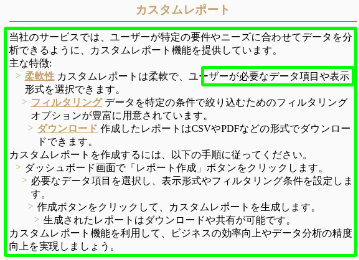
\includegraphics[width=1.0\textwidth]{image/6/app1.png}
    \caption{「カスタムレポート」が囲まれていない差分画像}
    \label{fig:app1}
\end{figure}

\begin{figure}[ht]
    \centering
    % 画像ファイル名とサイズを指定
    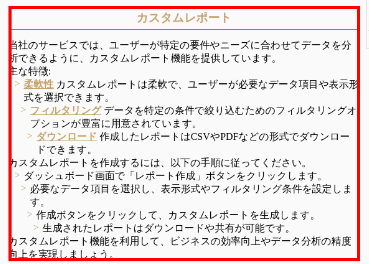
\includegraphics[width=1.0\textwidth]{image/6/app2.png}
    \caption{「カスタムレポート」が囲まれているHTMLコードによる変更箇所}
    \label{fig:app2}
\end{figure}

CaseBで被験者がレイアウトの不具合箇所を不足して検出したことについて、考察する。
BからDの被験者らは、レイアウトの不具合箇所として埋め込んだ画面要素のはみ出しに対して、
レイアウトの不具合箇所の検出不足があった。このことから、
画面要素のはみ出しのような見た目に変更が分かりづらい差分があった場合は、画像ベースの視覚的回帰テストでは検出しづらいことが分かった。

以上の評価結果の考察から、\toolName は、一般的な画像ベースの視覚的回帰テストと比較して、
HTMLコードに基づかない変更箇所を可視化できる視覚的回帰テストツールとして有用である。

\section{関連研究}\label{sec:relation_research}
本研究で試作した\toolName と、関連研究を比較する。
Haruto Tannoらは、領域ベースにおける視覚的回帰テストを行った\cite{RegionDetect}。
領域ベースで画像比較することで、本質的な差分と本質的でない差分を含んだ差分画像から、
本質的な差分のみを抽出できることを提案している。
また、塚越らは、GUI要素の階層構造を利用した差分検出方法を提案した\cite{GuiRetrExternal}。
\par
これらの既存研究は、手動で視覚的回帰テストを行う場合よりも、
画像比較による視覚的回帰テストを用いることにより、
レイアウトの不具合がないかどうかを効率的に見つけ出すことを提案している。
しかし、画像比較による差分をすべて抽出するため、抽出した差分には開発者の意図した変更も含まれてしまう。
そのため、HTMLコードの差分とレイアウトの差分における整合性の確認に時間がかかる。

これに対して、\toolName は、画像比較に基づく差分箇所から、HTMLコードの変更に基づく変更箇所を除いた、
レイアウトの不具合箇所のみを表示することができる。
そのため、\toolName は、既存研究と比較して、HTMLコードの差分とレイアウトの差分における整合性の確認にかかる時間の削減に
有用であるといえる。

\section{\toolName の問題点とその解決策}\label{sec:AWSEL_problems}
\toolName の問題点とその解決策について、以下に示す。
\begin{itemize}
    \item 入力対象とするWebページの画面サイズにおける問題:\\
          比較対象とするWebページの画面サイズと、テスト対象とするWebページの画面サイズが同じでないと、
          視覚的回帰テストを行うことができない。常に、画面サイズが同じ大きさだとは限らないため、画面サイズの差に閾値を設定することで、
          その閾値以内なら、画像の調整や比較方法を動的に変更できるようにする必要がある。
    \item 画像比較の制限に関する問題:\\
          一度にできる画像比較は、1回のみである。
          現在の\toolName では、一度に1回しかテストできないため、大規模な開発に有用性があると言えない。
          テスト対象とするWebページだけでなく、そのWebページから派生する別の開発Webページに対しても、視覚的回帰テストを行えるようにしなければ、
          実用的だと言えない。解決策として、Seleniumによるスクレイピング技術を用いたり、開発リポジトリをクローンしておくだけでそのリポジトリにおける開発Webページに対して、
          視覚的回帰テストを自動で実行できる機能を実装する必要がある。
    \item 入力対象とするWebページの背景における問題:\\
          背景が白地でなく、赤色や緑色であったりした場合に、適切に変更箇所に色付きの枠を付けることができない。
          現在の\toolName では、HTMLの変更箇所に赤枠や緑枠をつけて強調表示したり、画像比較で生成した差分画像に赤枠や緑枠をつけて強調表示したりしているが、
          テスト対象とするWebページの背景が白地でなく、赤や緑など強調する色付きの枠と同じであると、適切に強調することができない。
          解決策として、そのようなWebページは視覚的回帰テストの対象としない処理にするか、背景の色や画像内に多く含む色を検出し、その色と区別できる色で変更箇所を強調表示する必要があると考える。
          さらに、他の方法として、色付きの枠をつけて強調表示するのではなく、スライドバーで変更前画像と変更後画像のそのままの表示で切り替えられるようにすることが考えられる。
    \item 入力対象とするWebページのHTML構造における問題:\\
          複雑なHTML構造をしているWebページに対して、視覚的回帰テストがうまくできない。
          現在の\toolName では、HTML構造が一定の形式に沿っていないと適切にHTMLを解析することができず、視覚的回帰テストに用いることのできない、枠付きHTMLコードを生成してしまう。
          この解決策として、HTMLコードの解析をテキストベースで行うのではなく、DOM解析やより高度な解析技術を用いて、HTMLコードの解析が必要となる。
    \item 外部リンクの読み込みにおける問題:\\
          requestsによるHTMLコード取得では、CSSやJavaScriptがリンクで記述されていると、そのリンクを読み込むことができず、適切な枠付きHTMLコードを生成できない。解決策として、
          単一のHTMLコードだけでなく、そのHTMLに用いるCSSやJavascriptのファイルも取得できるようにする必要がある。
    \item レイアウトの不具合箇所の検出方法における問題:\\
          親子関係にある画面要素間に画面要素の重なりが発生しても、その箇所をレイアウトの不具合箇所として強調表示することができない。
          これが起こる原因は、画像比較で差分箇所に付ける枠と、HTML比較で変更箇所に付ける枠が5割以上重なっていない場合に、それらの枠をレイアウトの不具合箇所に付ける枠としているためである。
          解決策として、兄弟関係にある画面要素間に対応するだけでなく、様々なレイアウトの不具合箇所に対して適切な処理を施す必要がある。
\end{itemize}
